\documentclass[10pt]{article}

\usepackage[margin=1.3in]{geometry}
\usepackage{fancyhdr}
\usepackage{booktabs}
\usepackage[bookmarks, pdfauthor={Brian Kubisiak}]{hyperref}
\usepackage[parfill]{parskip}
\usepackage{todonotes}
\usepackage{tabularx}
\usepackage{siunitx}
\usepackage{tikz}
\usepackage{circuitikz}
\usepackage{fontspec}
\usepackage{listings}


% set options for fancy header
\pagestyle{fancyplain}
\date{}
\setlength{\headheight}{18pt}

% code input
\lstset{basicstyle=\ttfamily\footnotesize, numbers=left, frame=single, tabsize=4}

\setmainfont{Source Serif Pro}
\setmonofont{Source Code Pro}

\def\doctitle{EE 90 Project Documentation}
\hypersetup{pdftitle={\doctitle}}

\title{Smart Dog Bowl Using FFT Analysis of Dog's Bark}
\author{Brian Kubisiak \\ brian.kubisiak@gmail.com \\ MSC 606}

\begin{document}

\lhead{\large{Brian Kubisiak}}
\chead{\large{\doctitle}}
\rhead{\large{\today}}

\maketitle

\thispagestyle{empty}

\section{Motivation}
\label{sec:motivation}

In designing a smart dog bowl to open only for a specific dog, it is important
that method used for identifying the dog be very accurate; there should never be
a case where a dog is unable to access his food. Obvious approaches to this
problem would be to put some sort of identification tag on the dog's collar,
such as RFID or a modulated IR beacon.

However, these approaches can easily break down under fairly common
circumstances---IR must have a clear path to the sensor, and RFID depends on a
specific orientation. In addition, these approaches require the dog to be
wearing his collar, and---in the case of IR---the collar must be powered. I
believe that the most important part of this bowl is that a dog must never
approach his bowl, only to have it not open due to something blocking the
identification on his collar.

\section{Method of Approach}
\label{sec:method_of_approach}

To solve the problems described above, I have elected to identify the dog using
its bark. Just as humans each have a distinct-sounding voice, a dog's bark
contains a unique spectrum of frequencies. By analyzing these frequencies, I
believe that a system can be designed that will open for one dog's bark but not
another's.

The dog can never really ``lose'' his bark, so it is ideal in that the dog will
always be able to open the dish on his own. Additionally, in the case that an
error causes the dog to be misidentified, the dog will likely try again,
reducing the probability of error.

One disadvantage of this design is that the dog will have to be trained to bark
in order to open his food dish. However, this seems fairly easy, as teaching a
dog to ``speak'' is a fairly common trick. Another obvious disadvantage is that
the analysis will not get a distance measurement to the dog. In order to
overcome this, I will use ultrasonic ranging sensors to determine whether or not
the dog is within a \SI{1}{ft} radius.

\section{Operation}
\label{sec:operation}

My design comprises a microphone with an audio amplifier, triggering logic for
generating interrupts, an Arduino for performing the signal processing, and a
servo motor for opening the dog bowl.

All of the signal processing for this design will be performed on an Arduino
board. The processor will sample the dog's bark, then perform an FFT on the data
and compare it to save values. If the bark matches, the bowl will open.

There will be 4--6 ultrasonic proximity detectors to determine whether or not
there is an object within \SI{1}{ft} of the bowl. This will consist of an
ultrasonic range finder and circuitry comparing it to a reference range. This
detector will output a digital 1 if there is an object within a foot, and a 0 if
there is not.  Each range finder can detect in a \SI{15}{\degree} angle. By
putting 4--6 of these in a circle around the bowl, they should be able to detect
anything larger than a foot wide around the entire radius. More sensors can
easily be used, at an increased cost.

The microphone will output a simple analog signal into the Arduino. In addition,
some analog circuitry will be used to generate an interrupt whenever the analog
input reaches a certain threshold in order to allow the Arduino to idle at lower
power when data is not being read.

A block diagram for this design is shown in figure (\ref{fig:diagram}).

\begin{figure}[h]
    \centering
    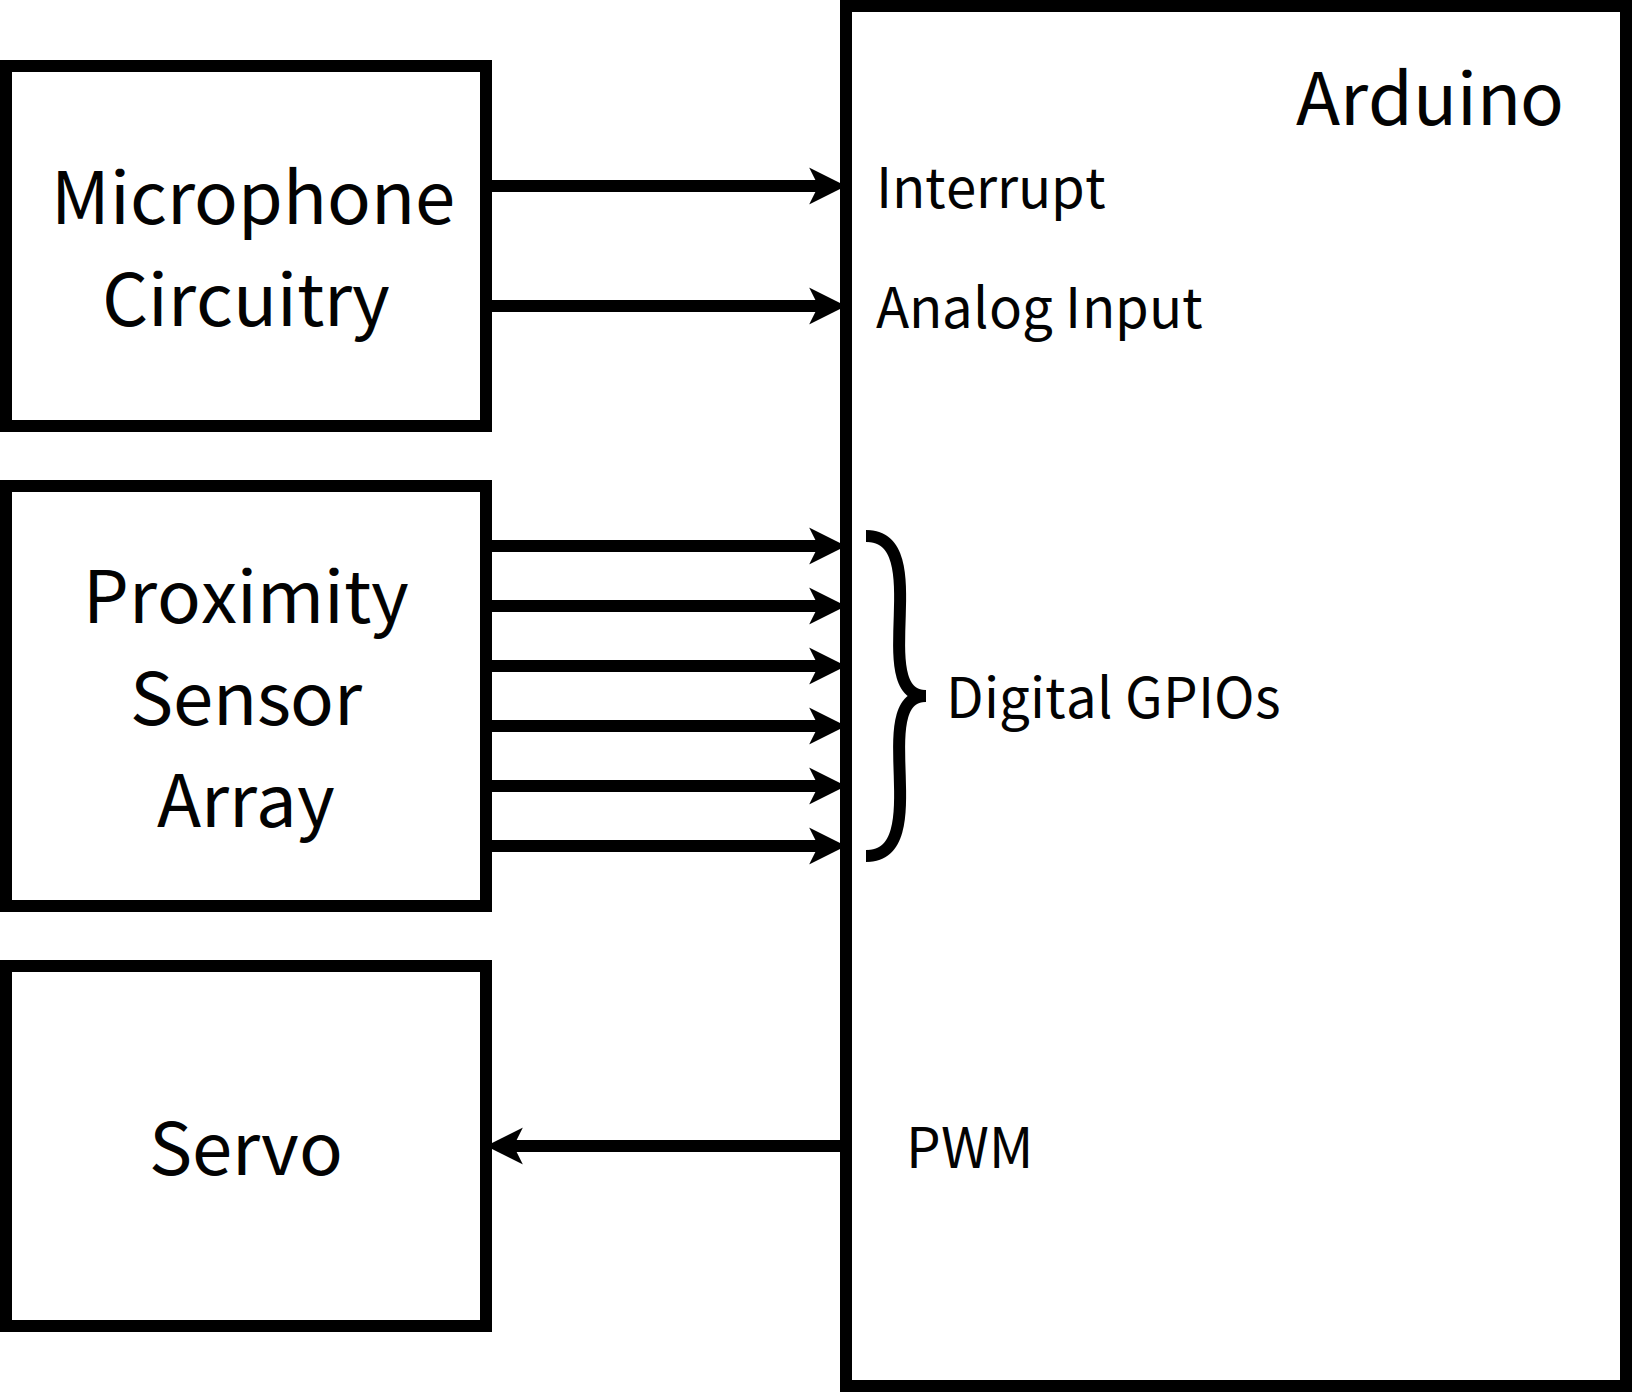
\includegraphics[width=0.4\linewidth]{sch/top-level.png}
    \caption{Top-level block diagram for the dog bowl.}
\label{fig:diagram}
\end{figure}

\subsection{Microphone Circuitry}
\label{sub:microphone_circuitry}

All of the microphone circuitry is detailed in figure~(\ref{fig:microphone}).

The microphone is powered from Vcc through a \SI{2.2}{\kilo\ohm} resistor,
as recommended in the data sheet. The signal is then lowpass-filtered before
being fed into the amplifier. The lowpass filter is designed with a corner
frequency of \SI{10}{\hertz} using R2 = \SI{100}{\kilo\ohm} and C1 =
\SI{1}{\micro\farad}. This will filter out the DC component without affecting
the AC signal.

The audio amplifier uses an op-amp with a single-sided supply in order to
amplify the input signal. The amplifier is arranged in a noninverting
configuration, with a total amplification factor of 560 (\SI{27.5}{\deci\bel}).
The resistor Rf can be adjusted as needed to change the amplification. Note
that the AC input may go below ground, but this will be clipped by the
amplifier.

The output of the amplifier is then fed directly into the ADC on the Arduino
board. This amplified signal is also fed into the comparator U2 in order to
generate an interrupt to tell the Arduino to begin recording the audio. The
trigger level is set with R4 and R5. I have found that a level of around
\SI{1.7}{\volt} works well. This interrupt trigger is fed into a GPIO pin on the
Arduino to generate an interrupt.

\begin{figure}[h]
    \centering
    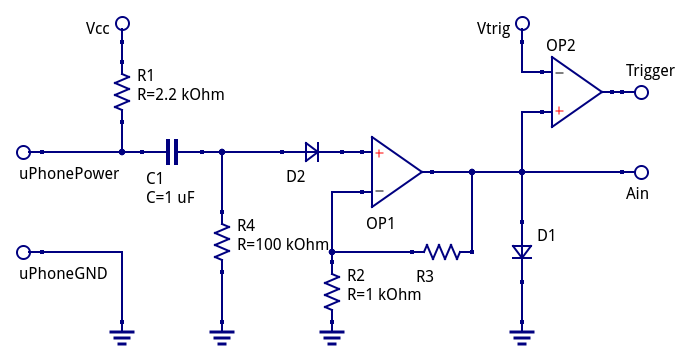
\includegraphics[width=0.8\linewidth]{sch/microphone.png}
    \caption{Microphone amplifier and trigger generator.}
\label{fig:microphone}
\end{figure}

\section{Schedule}
\label{sec:schedule}

For the duration of this term, I will attempt to observe the following schedule.
Note that some of the tasks near the end of the term are simpler and some can be
eliminated entirely if I lack the time to implement them. This allows for some
flexibility in case I fall behind in the beginning of the term.

\setlength\extrarowheight{5pt}
\begin{tabularx}{\textwidth}{c X}
    Week & Tasks \\
    \midrule
    03/29 & This is the first week of the term. In this week, I will write my
    project proposal, including a block diagram demonstrating my general plan
    for the term. \\
    04/05 & For this week, I will draw schematics for my circuitry. Since a
    large part of the project is on the Arduino, the schematics will be fairly
    small, elaborating the comparators for the rangers and the triggering
    circuit. At the end of the week I will order all the parts I cannot get from
    the stockroom. \\
    04/12 & While waiting for the parts to be shipped, I will begin writing the
    code for the Arduino board. This includes coding an FFT and code for
    comparing the spectrum to a pre-recorded spectrum. Time-permitting, I will
    also write code for interfacing with the hardware. \\
    04/19 & Once my parts arrive, I will breadboard the microphone triggering
    circuit and thoroughly test it. I will also make sure that the microphone
    works with the Arduino board. \\
    04/26 & This week, I will breadboard the ranging circuit and ensure that it
    will work as a proximity sensor. The midterm demo is also during this week. \\
    05/03 & Now that the hardware circuits should be working, I will write the
    hardware interface code and test the circuits with the Arduino. \\
    05/10 & All hardware and software should be debugged at this point. During
    this week, I will construct the final circuitry on a prototyping board. \\
    05/17 & At this point, the majority of the work is done. This week, I will
    wire the servo and test to make sure I can control it properly. I will also
    design the hardware I will use for the bowl. \\
    05/24 & During this week, I will build the bowl and package the electronics. \\
    05/31 & The project should be mostly done at this point. During this week, I
    will finish up the packaging and the documentation for the project. \\
    06/07 & Final demonstration.
\end{tabularx}

\end{document}

